\documentclass[11pt]{article}

\usepackage[dvinames]{xcolor}
\usepackage{microtype}
% Measurements are taken directly from the guide
\usepackage[top=0.75in,left=0.75in,bottom=0.75in,right=0.75in]{geometry}
\usepackage{graphicx}

\usepackage{lipsum}
\usepackage[absolute]{textpos}
\usepackage{tikz}
\usepackage{url}
\usepackage{titling}
\usepackage{lmodern}
\usepackage{listings}
\usepackage{enumerate}
\usepackage{wasysym}
\usepackage{amsfonts}
\usepackage{url}

% No paragraph indentation
\parindent0pt
\setlength{\parskip}{0.8\baselineskip}




%\setlength{\droptitle}{-1cm}

\preauthor{\begin{center}
            \large \lineskip 5.5em%
            \vspace{-0.7cm}
            \begin{tabular}[t]{c}}
                
                
                
\postdate{\par\end{center}
            \vspace{-2cm}
         }

\title {CSE 30: Data Structures\\Laboratory 10}
\author {Spring 2019}
\date {}


%\renewcommand{\labelitemi}{\Large$\circ$}


\makeatletter
\ifcase \@ptsize \relax% 10pt
  \newcommand{\miniscule}{\@setfontsize\miniscule{4}{5}}% \tiny: 5/6
\or% 11pt
  \newcommand{\miniscule}{\@setfontsize\miniscule{5}{6}}% \tiny: 6/7
\or% 12pt
  \newcommand{\miniscule}{\@setfontsize\miniscule{5}{6}}% \tiny: 6/7
\fi
\makeatother

\lstset{language=C++,
                basicstyle=\ttfamily,
                keywordstyle=\color{blue}\ttfamily,
                stringstyle=\color{red}\ttfamily,
                commentstyle=\color{green}\ttfamily,
                morecomment=[l][\color{magenta}]{\#},
				showstringspaces=false
}




\newcommand{\progtotal}{15}
\newcommand{\abstotal}{22}
\newcommand{\encaptotal}{15}
\newcommand{\ooptotal}{20}

\newcommand{\bonuspoints}{2}

\newcommand{\total}{\the\numexpr\progtotal+\abstotal+\encaptotal+\ooptotal-\bonuspoints\relax}

\newcommand{\available}{\the\numexpr\total+\bonuspoints\relax}

\begin{document}


% -------------------------------------------------------
\begingroup
\fontsize{10pt}{12pt}\selectfont
\begin{textblock*}{4.5in}(0.75in,1in)
	\hrule
	\vspace{-0.25cm}
	\miniscule \textls[-50]{BERKELEY} \tiny $\cdot$ 
	\miniscule \textls[-50]{DAVIS} \tiny $\cdot$
	\miniscule \textls[-50]{IRVINE} \tiny $\cdot$
	\miniscule \textls[-50]{LOS ANGELES} \tiny $\cdot$
	\miniscule \textls[-50]{MERCED} \tiny $\cdot$
	\miniscule \textls[-50]{RIVERSIDE} \tiny $\cdot$
	\miniscule \textls[-50]{SAN DIEGO} \tiny $\cdot$
	\miniscule \textls[-50]{SAN FRANCISCO}
	\vspace{0.15cm}
	\hrule
\end{textblock*}
\endgroup
\begin{textblock*}{6.375in}(0.75in,0.55in)   % 6.375=8.5 - 1.5 - 0.625
    \large UNIVERSITY OF CALIFORNIA, MERCED
	\normalsize
\end{textblock*}

\begin{textblock*}{1in}(5.3in,0.65in)   % 6.375=8.5 - 1.5 - 0.625
    
\includegraphics[width=0.85in]{seal.pdf}
\end{textblock*}


\begin{textblock*}{1.5in}(6.2in,1in)
	\hrule
	\vspace{-0.25cm}
	\miniscule $\;$ \textls[-50]{SANTA BARBARA} \tiny $\cdot$
	\miniscule \textls[-50]{SANTA CRUZ}
	\vspace{0.15cm}
	\hrule
\end{textblock*}

\maketitle

\section*{Introduction}
This lab is based on the Kevin Bacon game, which itself is based on the ``Six Degrees of Separation'' concept. The idea behind six degrees of separation is that any two people on earth are connected to each other by at most 6 social connections. Basically if you consider:

\begin{enumerate}
    \item your friends,
    \item your friends' friends,
    \item your friends' friends' friends,
    \item your friends' friends' friends' friends,
    \item your friends' friends' friends' friends' friends,
    \item your friends' friends' friends' friends' friends' friends,
\end{enumerate}    

then you have covered every person on earth.

The Kevin Bacon game is a similar concept but with movies and actors. Two actors are directly related together if they have appeared in the same movie. They are separated by one degree if they have not appeared in the same movie, but they have appeared in two different movies with the same mutual co-star.

If you consider the network of actors in Figure~\ref{imdb}. You can see for example that Harrison Ford is connected to Mark Hamill because they both appeared in Star Wars. Harrison Ford is also connected to Sean Connery because they were in Indiana Jones together. (To be precise, that refers to Indiana Jones and the Last Crusade, but the label on the edge would have been too long.)

Now, even though Mark Hamill and Sean Connery have not appeared in the same movie together (at least according to our records in Figure~\ref{imdb}), they are still connected through Harrison Ford. We can build a chain that looks like this:

\begin{center}
    \texttt{Mark Hamill (Star Wars) Harrison Ford (Indiana Jones) Sean Connery}
\end{center}

There are many other possible chains in this network, Marlon Brando to Robert De Niro, via Al Pacino, and many others. There are some actors who are not connected to anyone, like John Cena (once again as far as we know from the information in Figure \ref{imdb}).



\begin{figure}[!htbp]
    \begin{center}
        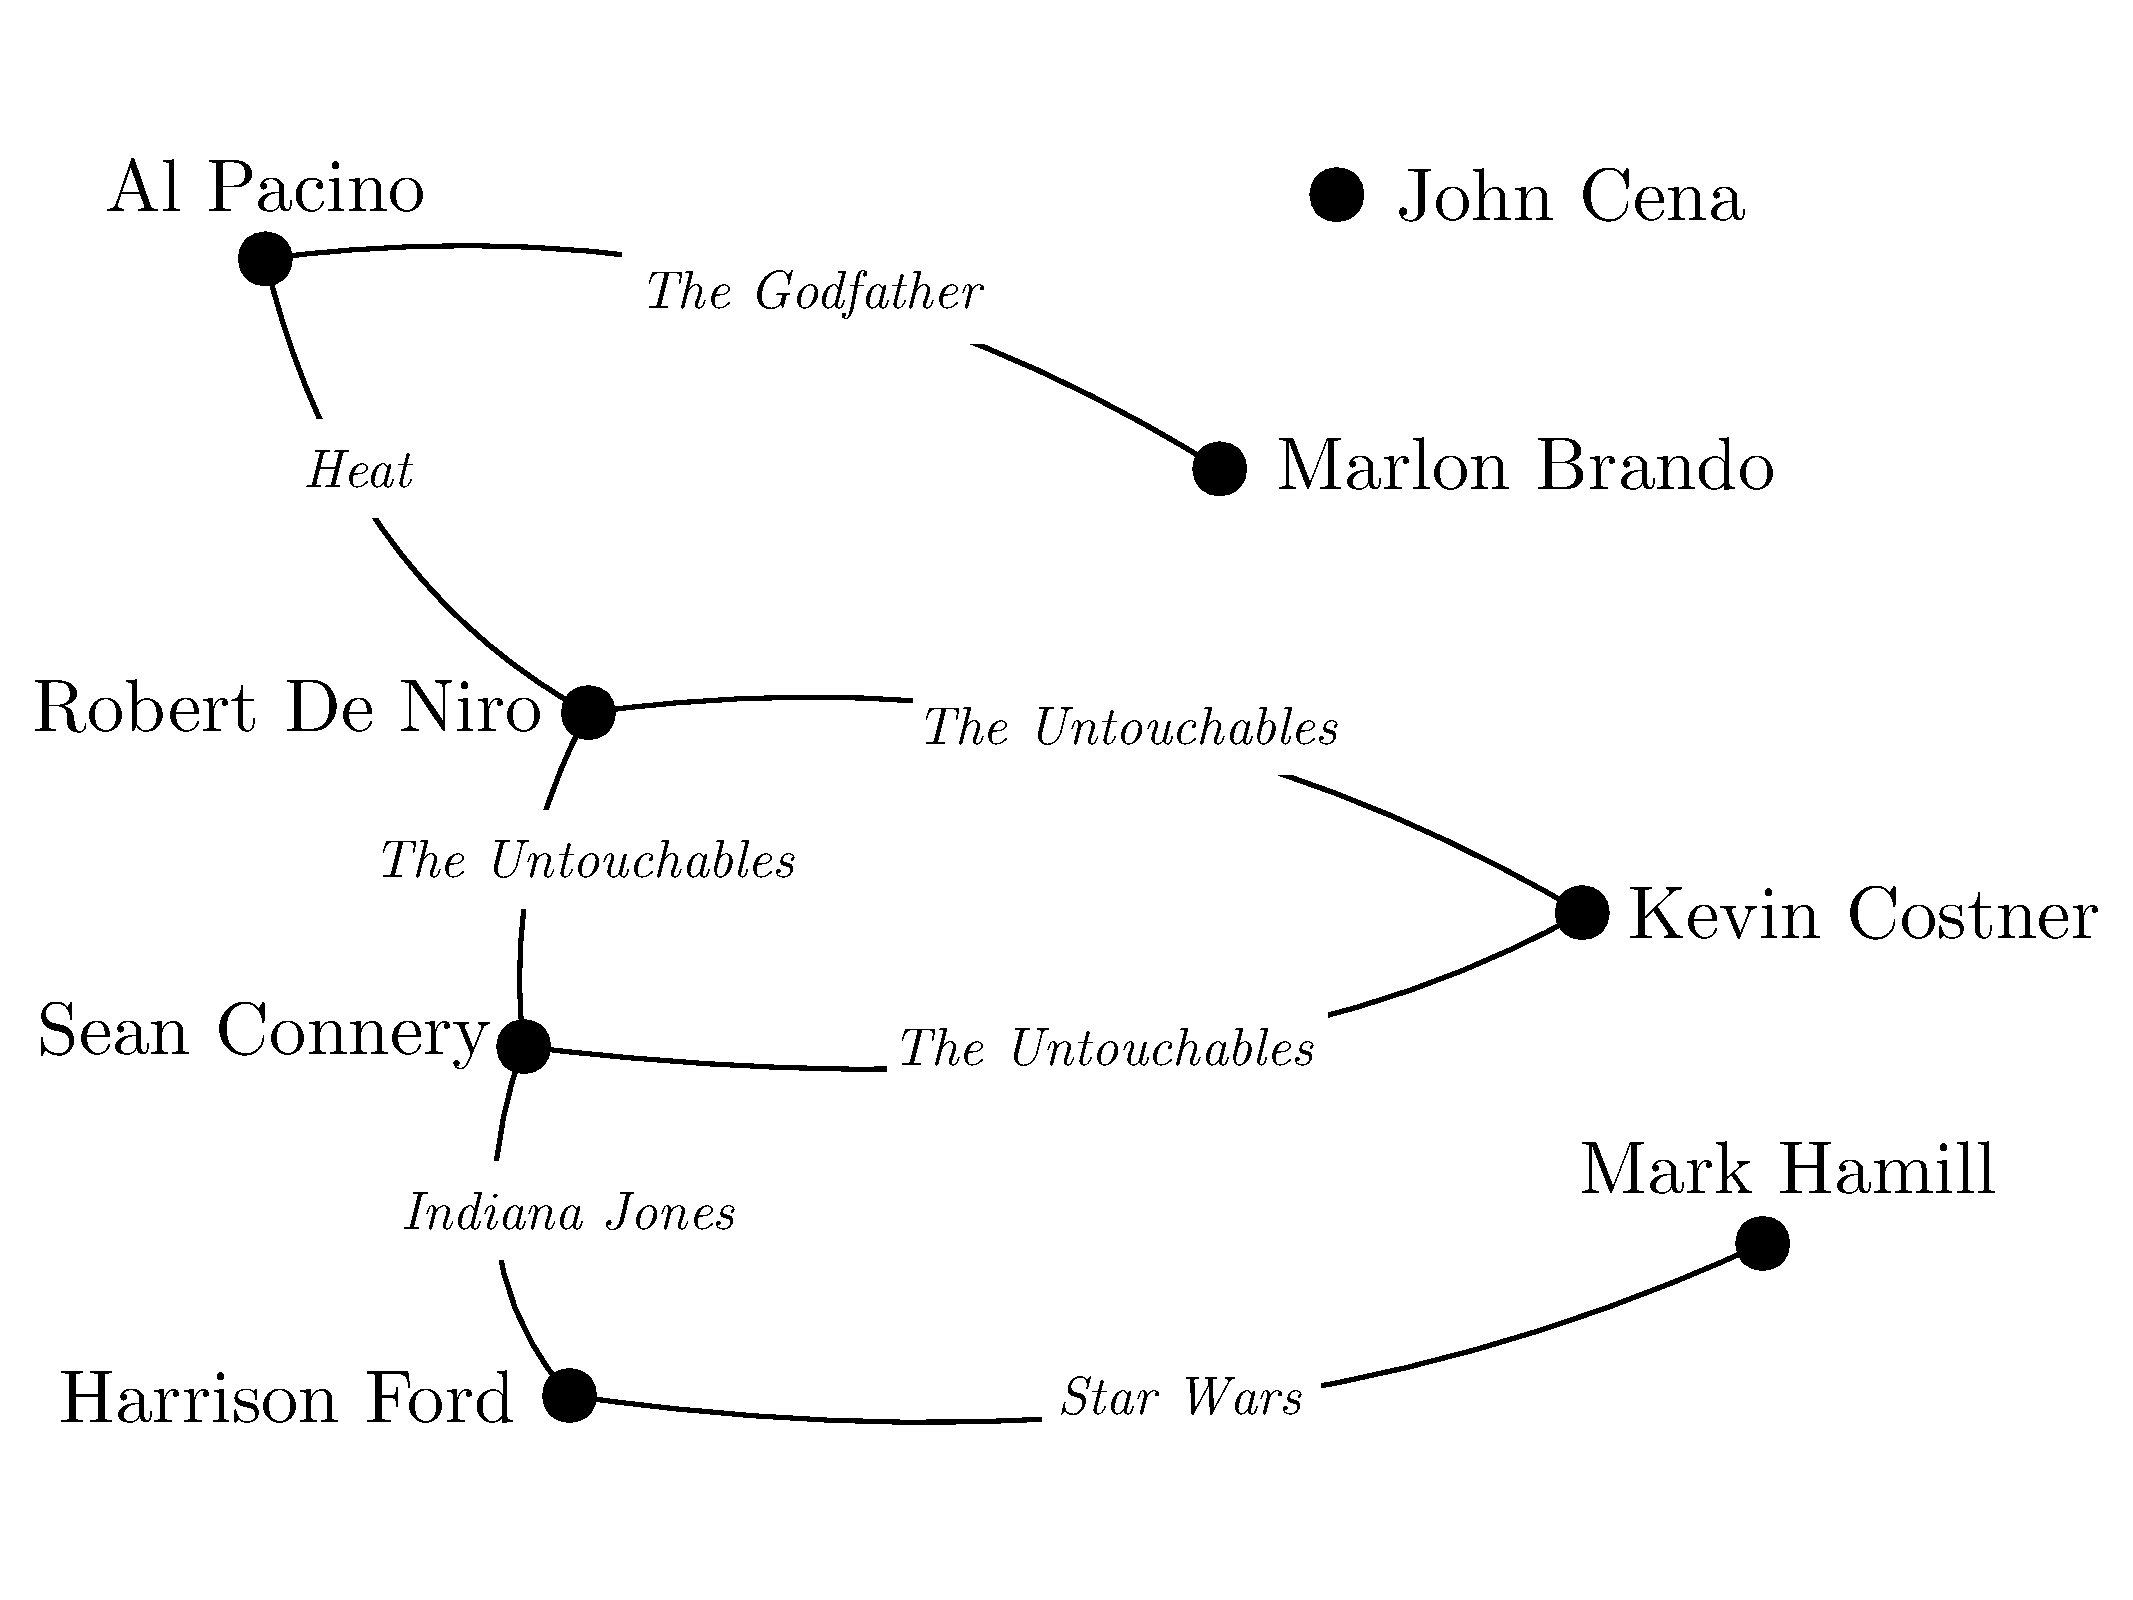
\includegraphics[scale=0.4]{imdb.pdf}
    \end{center}
    \caption{A Sample Network of Actors and Movies}
    \label{imdb}
\end{figure}

If you look at the file \texttt{KB.cpp}, it represents the information from Figure~\ref{imdb} as a graph, and then it checks to see if there is a chain between two given actors. The expected output is shown in the file. The definition of the \texttt{Graph} data structure and all its algorithms has been omitted, and it is your task to provide it, so that the file \texttt{KB.cpp} compiles and runs correctly.

You can use the demo files from class that can be found in the \texttt{Graphs} folder. The difference is that in the demo files, vertices were labelled with an integer, and now we need them to be labelled with a string. The other difference is that in the class demo, there were no edge labels, and now we need to incorporate them as the movie names are the edge labels in our graph.

Hint: To find a chin between 2 actors, just do a Breath-First Search from one to the other and output the resulting path.

Upload your completed \texttt{KB.cpp} file to CatCourses.

\end{document}